\documentclass[english,12pt]{aghthesis}

\usepackage[T1]{fontenc}
\usepackage[utf8]{inputenc}
\usepackage{upgreek}
\usepackage{polski}
\usepackage{url}
\usepackage{graphicx}
\usepackage{float}
\usepackage{hyperref}
\hypersetup{colorlinks,breaklinks,urlcolor=black,linkcolor=black,pdfborderstyle={/S/U/W 1}}
\usepackage{tikz}
\usetikzlibrary{positioning}
\bibliographystyle{ieeetr}

\newcommand{\tech}[1]{\textbf{#1}}

\author{Antoni Mleczko \\ Maciej Mionskowski}

\titlePL{Interaktywna wizualizacja instrukcji składania Origami z elementami symulacji fizyki papieru}
\titleEN{Interactive visualization of Origami folding with elements of paper physics simulation}

\fieldofstudy{Informatyka}

\supervisor{dr inż. Witold Alda}

\date{\the\year}

\begin{document}
\setlength{\parskip}{0pt} % 1ex plus 0.5ex minus 0.2ex}
\setlength{\parindent}{0pt}

\maketitle

\tableofcontents
\clearpage

\section{\SectionTitleProjectVision}
\label{sec:vision}
\subsection{Problem characteristics}
Origami has been around for a long time. It originated in China and Japan, roughly at the same time, from where it 
spread all around the world\cite{wiki:history-of-origami}. 
Origami is recognized as the art of paper folding.
Although known for centuries, it exhibits properties that are applicable 
in many different contemporary contexts, e.g.
space exploration\cite{origami-in-orbit}, or deploying solar arrays\cite{solar-panel-origami}.
It has recently started to attract attention among scientists and engineers.
Researchers are now recognizing material folding as a distinct
branch of computer science, known as \hyperref[dictionary:computational-origami]{\textit{computational origami}}.
The field has seen tremendous development in the past couple of decades.
Being such a broad topic, it is not surprising that there are numerous open problems\cite{mit-open-problems} and on-going research.

\medskip

While beginners fold origami following step-by-step instructions,
more advanced origamists would use \hyperref[dictionary:crease-pattern]{\textit{crease patterns}}
to form the \hyperref[dictionary:folded-state]{\textit{folded state}}.
The process of origami creation consists of two stages: \textit{design} and \textit{folding}.
The former is a reference to the \textit{crease pattern} creation, and the latter is the process of the actual folding.

\begin{figure}[H]
\caption{A crease pattern for a popular origami model, a crane.\label{fig:creasepattern}}
  \centering
    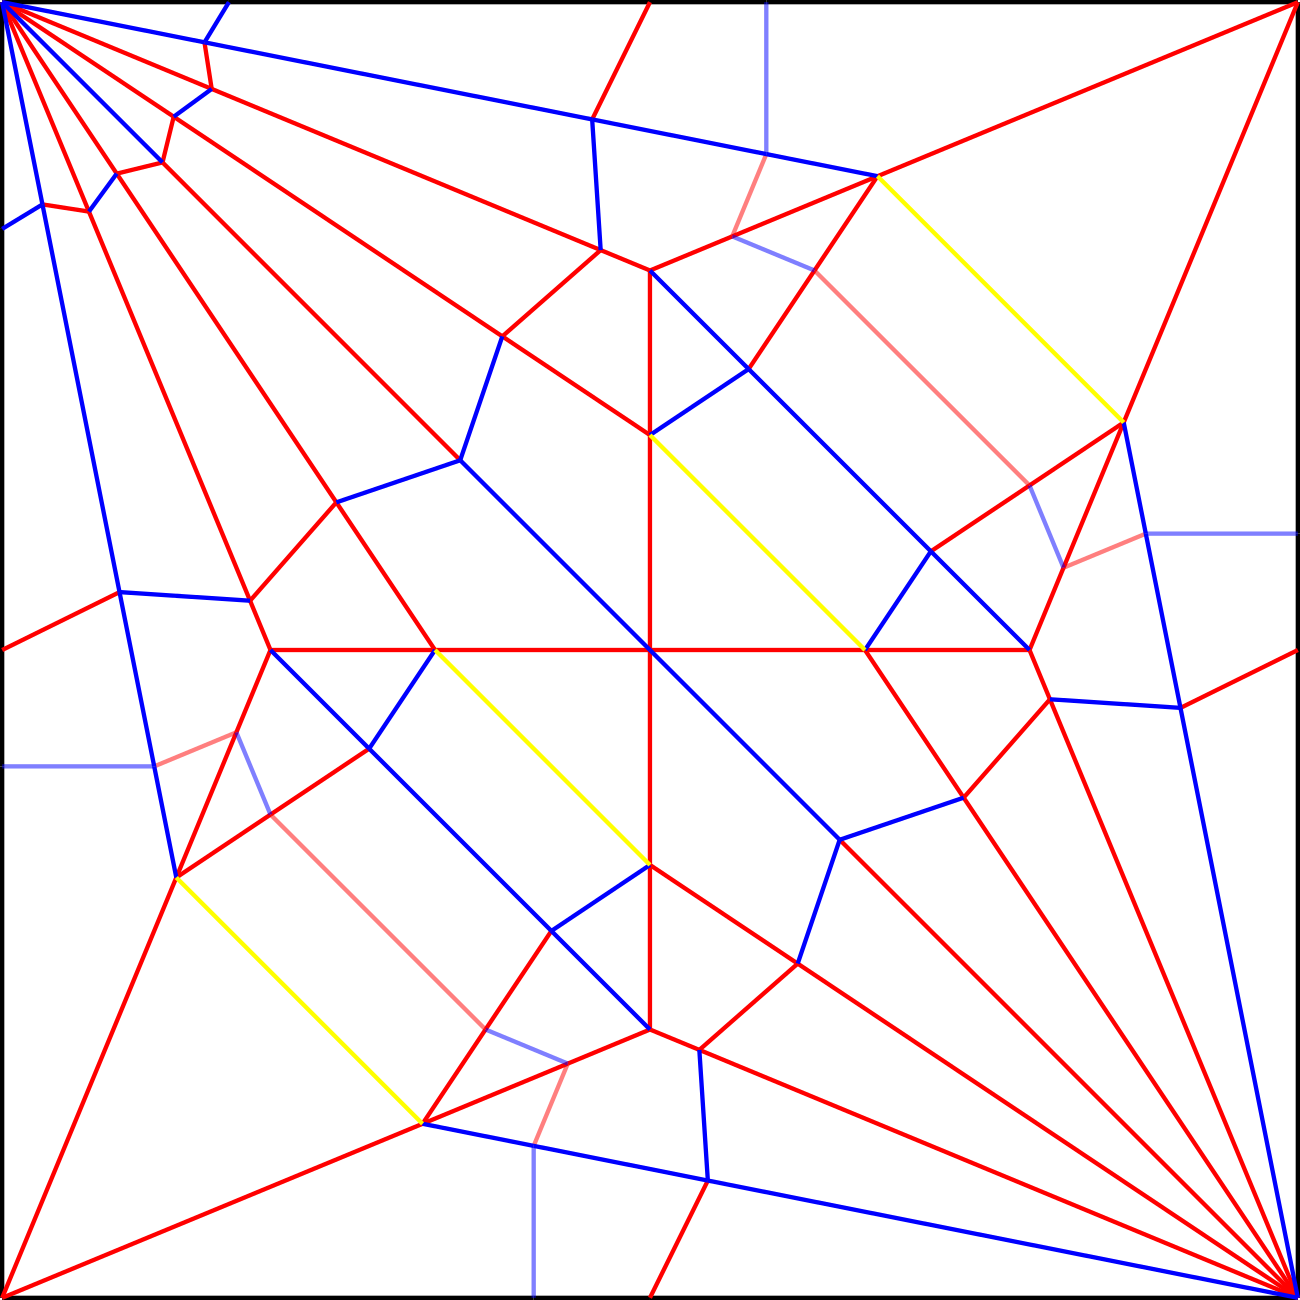
\includegraphics[width=0.8\textwidth]{assets/crane-crease-pattern.png}
\end{figure}

\subsection{Motivation}

Even though origami might seem to be a child's play, at times
people would get discouraged whilst following the origami instructions due to
the lack of details they expose.

We would like to provide a way, for beginners and advanced origamists alike,
to visualize the folding process step by step.
While there exist some programs aiding the process of design\cite{app:treemaker}\cite{app:omto}\cite{app:origami-draw}, there is no satisfactory solution 
that would present the process of folding the way it would be carried out manually.

We have evaluated existing products, and the one that resembles 
what we would like to achieve the most\cite{origami-simulator} provides a way to load a crease pattern
and view the folding process. 
However, it goes immediately from a flat sheet of paper to the folded figure, skipping all the steps
that would be required while folding the figure by hand.
It also bypasses some physical properties that we would like to achieve, such as the fact that the
paper should not interpenetrate itself.


\begin{figure}[H]
\caption{Origami simulator by Amanda Ghassaei}
  \centering
    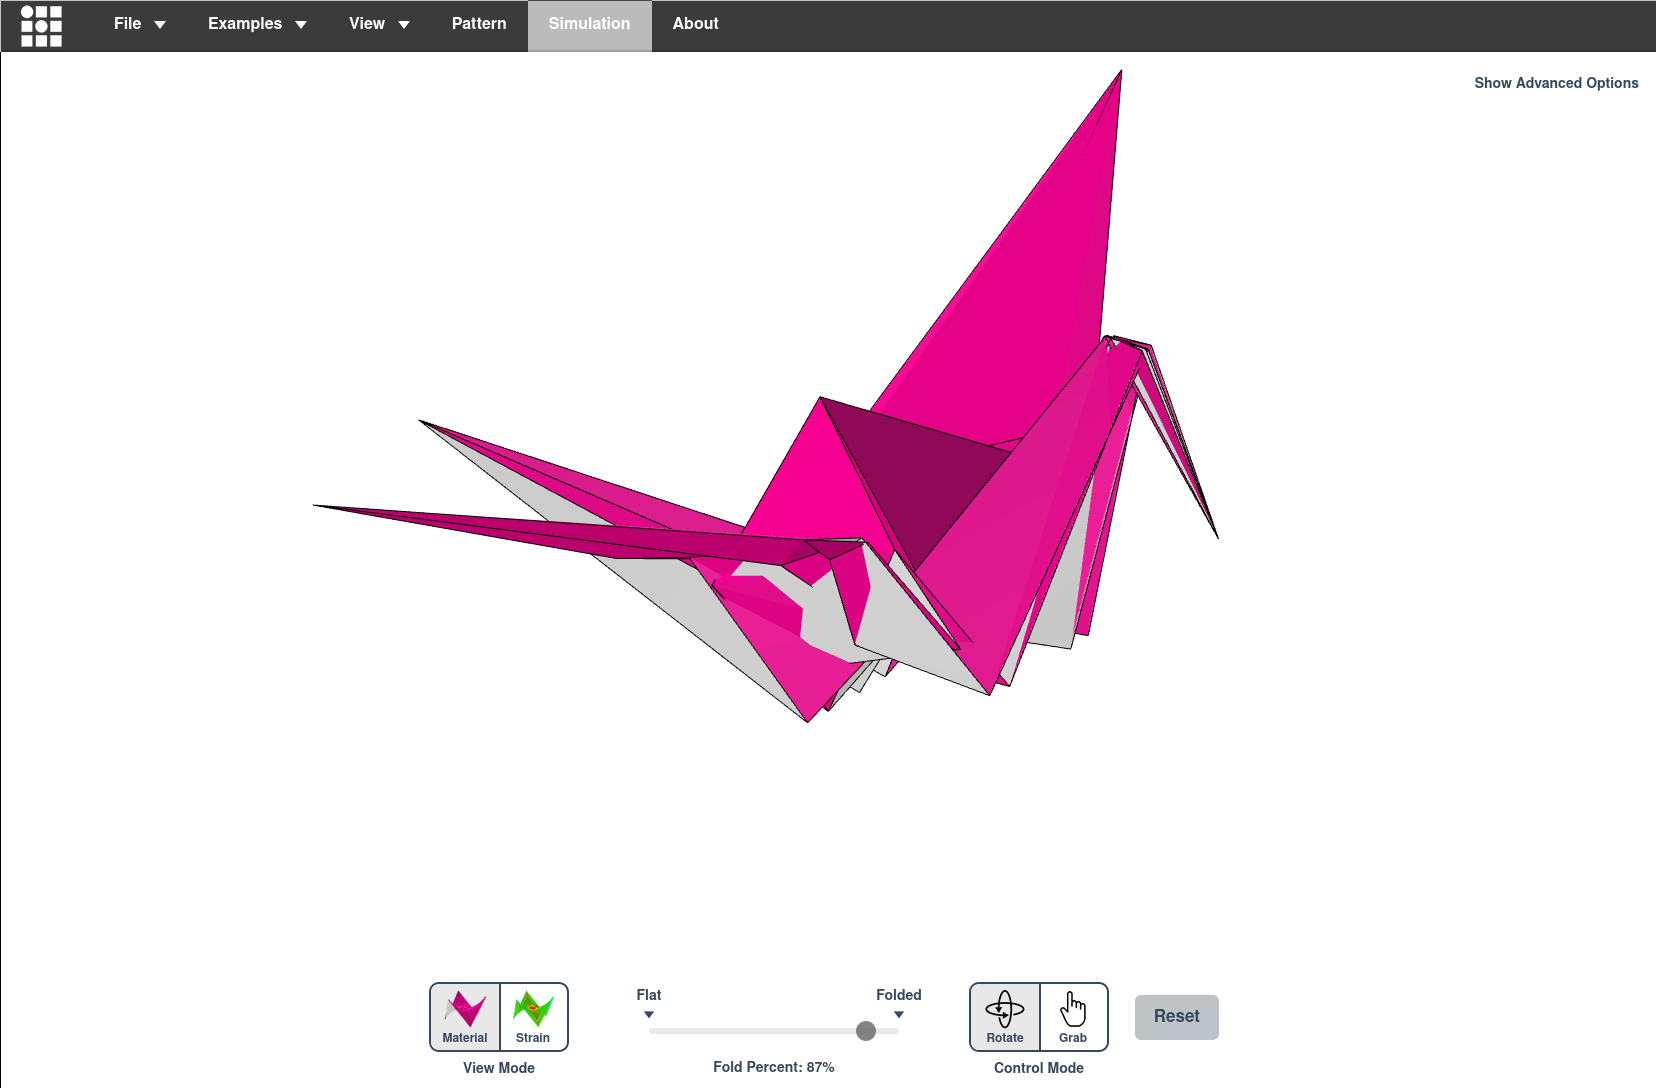
\includegraphics[width=\textwidth]{assets/origami-simulator.png}
\end{figure}

\clearpage 

\subsection{Product Vision}

\subsubsection{Functionality}

Our main goal is to create a platform that would allow visualisation of the origami folding process in a 3D space.
It would be possible to see how the figure folds at each step by playing an animation of the transition.

The inseparable component of the system would be a file format describing the folding sequence necessary to complete the origami figure.\\

The users in our system would at least be able to:
\begin{itemize}
	\item load a folding instruction,
	\item choose a step they want visualized,
	\item rotate the scene,
    \item zoom in and out,
	\item move around the scene,
	\item pause the animation at any time, and move back and forth.
\end{itemize}

\subsubsection{Technology}

Our application will consist of two layers -- backend and frontend.

The backend part will be responsible for storing user files and turning Instructions into animated Guides.
The frontend part will handle user interactions and 3D visualisations.

We have decided to use well-known and widely spread technologies.
For the backend part we will take advantage of \tech{Python} language with \tech{Django} framework.
As a data storage, we are going to incorporate \tech{PostgreSQL}.

For the frontend, we will use \tech{JavaScript} with \tech{React} for building the user interface.
The 3D rendering will be performed using \tech{Three.js} library that is built on top of \tech{WebGL} renderer.

\begin{figure}[H]
	\caption{Technology stack}
	\centering
	\begin{tikzpicture}
	\node (backend) at (0,0) [draw,thick,minimum width=4cm,label=north west:Backend] {
		
\includegraphics[width=.15\textwidth]{assets/python.png}
		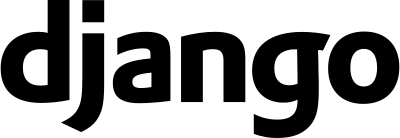
\includegraphics[width=.15\textwidth]{assets/django-logo.png}
	};
	\node[below = of backend] (frontend) [draw,thick,minimum width=4cm, label=north west:Frontend] {
		
\includegraphics[width=.12\textwidth]{assets/javascript-logo.png}
		
\includegraphics[width=.12\textwidth]{assets/react-logo.png}
		
\includegraphics[width=.23\textwidth]{assets/three-js-logo.png}
	};
	\draw[<->,thick] (backend.south) -- (frontend.north);
	\end{tikzpicture}
\end{figure}


\subsection{Feasibility Study}

Both \tech{Python} and \tech{JavaScript} are widely spread and actively maintained.
There is a strong community surrounding both of them.
\tech{Three.js} is the most popular library for 3D \tech{WebGL} rendering.

Therefore, we are not expecting problems connected with the tools we have selected.

Since the project will require a lot of knowledge from the \textit{computational origami}
field, we will have to research the existing materials on this topic.
The most promising resources seem to be the MIT course by
Eric Demaine\cite{mit-course} and a book co-authored by the same person -- \textit{Geometric Folding Algorithms: Linkages, Origami, Polyhedra}\cite{origami-book}.
Various available papers might come in handy as well, especially the ones regarding software implementations of origami folding algorithms.


\subsection{Threat Assessment}

Playing with the intersection between reality and computer science has always been a challenging task.
As the field of \textit{computational origami} is relatively young\cite{recent-results-in-computational-origami:paper}, there are still many obstacles to overcome.
As of now, the mathematical rules governing the origami folding are not fully developed.
On top of it, we are going to tackle a problem that has not been widely discussed.

Taking all of that into account, we foresee many challenges along the way, such as:

\begin{itemize}
	\item NP-hardness - some problems that we will face are proved to be NP-hard.
		Computing layer ordering based on a crease pattern is an example of such a problem.
		We will have to overcome them, either by using approximate methods or coming up with solutions that will avoid them.

	\item Physical properties of paper - should we support more complex physical properties,
		there are many features that would require a separate set of computations simulating paper physics, e.g.
		\begin{itemize}
			\item inflating,
			\item curving,
			\item cutting.
		\end{itemize}

	\item Performance -- web browsers are still not fully optimized to carry out 3D computations and render 3D graphics in real time.
		The system will have to be highly optimized in order to be usable.
		
	\item Mathematics -- we have little experience writing complex simulations utilizing complicated mathematical formulas.
		Even modelling a simple paper fold requires a lot of knowledge on different physical properties and frameworks that one could use.

	\item 3D graphics -- we have some experience working with 3D, however only from the user perspective.
		We have little experience in creating 3D graphical software.

\end{itemize}

Having said that, we believe we are capable of undertaking this problem and providing a solution to it.
Albeit challenging, it is rewarding especially in terms of projected business value and gained expertise.

\subsection{Dictionary}\label{dictionary}

\begin{description}
	\item[computational origami] \label{dictionary:computational-origami} -- a recent branch of computer science studying efficient algorithms for solving paper-folding problems.\cite{recent-results-in-computational-origami:paper}
	\item[crease] -- a line segment, along which a sheet of paper folds.
	\item[crease pattern] \label{dictionary:crease-pattern} -- a pattern of lines formed by creases that is created after unfolding the origami flat. For an example see figure \ref{fig:creasepattern}.
	\item[folded state] \label{dictionary:folded-state} -- An assembled origami model. Or alternatively, a sheet of paper folded along the crease pattern.
	\item[mountain] -- a fold of paper along the crease, such that the facets on the sides of the crease are facing downwards.
					\begin{figure}[H]
						\caption{Example of a mountain crease}
						\centering
						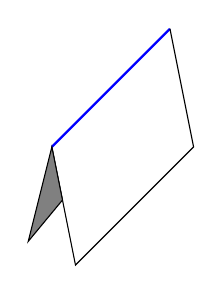
\begin{tikzpicture}[scale=1.5]
							\draw[blue, thick] (0,0) -- (1,1);
							\draw (1,1) -- (1.2, 0) --  (0.2, -1) -- (0,0);
							\filldraw[fill=gray] (0, 0) -- (-0.2, -0.8) -- (0.09, -0.45) -- cycle;
						\end{tikzpicture}
					\end{figure}
	\item[valley] -- A fold of paper along a crease, such that the facets on the sides of the crease are facing upwards.
					\begin{figure}[H]
						\caption{Example of a valley crease}
						\centering
						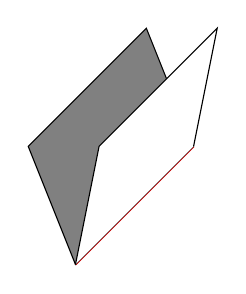
\begin{tikzpicture}[scale=1.5]
							\draw[red, thick] (0,0) -- (1,1);
							\filldraw[fill=gray] (0, 0) -- (-0.4, 1) -- (0.6, 2) -- (1, 1) -- cycle;
							\filldraw[fill=white] (1,1) -- (1.2, 2) --  (0.2, 1) -- (0,0);
						\end{tikzpicture}
					\end{figure}
	\item[mountain-valley assignment] -- an assignment of mountain or valley to the creases on the crease pattern.
	\item[.fold file] -- a file that conforms to the FOLD\cite{fold:paper} specification.
	\item[Instruction] -- a \textit{.fold} file created by a user, representing a sequence of steps required to
		fold a sheet of paper into a complete origami figure.
	\item[Transition] -- a folding animation played between two steps.
	\item[Guide] -- a set of all Transitions derived from an Instruction. Can be represented using a \textit{.fold} file.
	\item[Model] -- 3D representation of an origami figure. 
	\item[FPS] -- frames per second.
	\item[target angle] -- the supplement of the dihedral angle between the two neighbouring faces,
		towards which the faces should fold.
\end{description}




\clearpage

\section{\SectionTitleScope}
\label{sec:functionality}
\subsection{System actors}

Based on the requirements analysis, we have determined two types of actors in our system:

\begin{description}
	\item[Folder] \label{actors:folder} - A person who carries out the most important functionality in our system,
		that is - folds origami figures following the provided interactive instruction.
		This person does not need to have any special knowledge about origami creation nor the simulation process.
	\item[Designer] \label{actors:designer} - A person who is responsible for providing folding instructions
		for other users (\textit{folders}).
		A Designer is required to have basic knowledge about origami construction
		and interaction with the system to be able to create and upload an Instruction.
\end{description}

\newcommand{\requirement}[2]{\item #2. (#1)}
\subsection{Functional requirements}
\label{section:functional-requirements}

We define functional requirements for the system as User Stories grouped by actor type.
They have a priority assigned to them that ranges from 1 to 3. Where:

\begin{enumerate}
	\item[(3)] high priority - a feature required for the system functionality 
	\item[(2)] medium priority - a feature that is important, but not essential for the system functionality
	\item[(1)] low priority - a feature that is nice to have, but not required 
\end{enumerate}

\subsubsection{Folder user stories}
As a folder I am able to\ldots
\begin{enumerate}
	\requirement{3}{load an Instruction}
	\requirement{3}{view the 3D representation of the Instruction step}
	\requirement{3}{switch to the next step in the Instruction}
	\requirement{3}{switch to the previous step in the Instruction}
	\requirement{3}{see the Transition between two Instruction steps}
	\requirement{2}{pause the Transition at any time}
	\requirement{2}{rewind the Transition}
	\requirement{2}{forward the Transition}
	\requirement{3}{rotate the Model in 3D space}
	\requirement{3}{zoom the Model in and out in 3D space}
	\requirement{1}{see creases of the Model} 
	\requirement{2}{distinguish paper's top and bottom sides} 
	\requirement{1}{change the color of the paper side} 

	\requirement{3}{navigate between simulator and community views} 
	\requirement{3}{view Instructions uploaded by other users} 

	\requirement{3}{create an account} 
	\requirement{3}{log into the system} 
	\requirement{3}{reset the password} 
	\requirement{2}{change the password} 
	\requirement{2}{delete the account} 
	\requirement{2}{save another user's Instruction in my account} 
	\requirement{1}{mark a saved Instruction as folded} 
\end{enumerate}

\subsubsection{Designer user stories}
As a designer I am able to\ldots
\begin{enumerate}
	\requirement{3}{upload an Instruction}
	\requirement{3}{view my Instructions}
	\requirement{3}{delete my Instructions}
	\requirement{3}{update my Instructions}
	\requirement{1}{mark my Instructions as public or private}

	\requirement{1}{visually design an Instruction}
	\requirement{1}{save a designed Instruction}
\end{enumerate}

\subsection{Non-functional requirements}

We have deduced the following non-functional requirements that our system
needs to fulfill in order to meet the client's expectations.

\begin{enumerate}
	\requirement{3}{Anyone with an up to date web browser is able to use the application}
	\requirement{3}{The application must be reachable under a public address}
	\requirement{1}{All system components can be run on separate machines}
	\requirement{2}{Transitions should be played in at least 24 FPS on modern hardware}
	\requirement{1}{User should be able to use the application on mobile devices}
\end{enumerate}

\subsection{UI wireframes}

Based on the requirements, we have created the following UI wireframes that
present the most important parts of our system.


\begin{figure}[H]
\caption{Guide Viewer view}
  \centering
    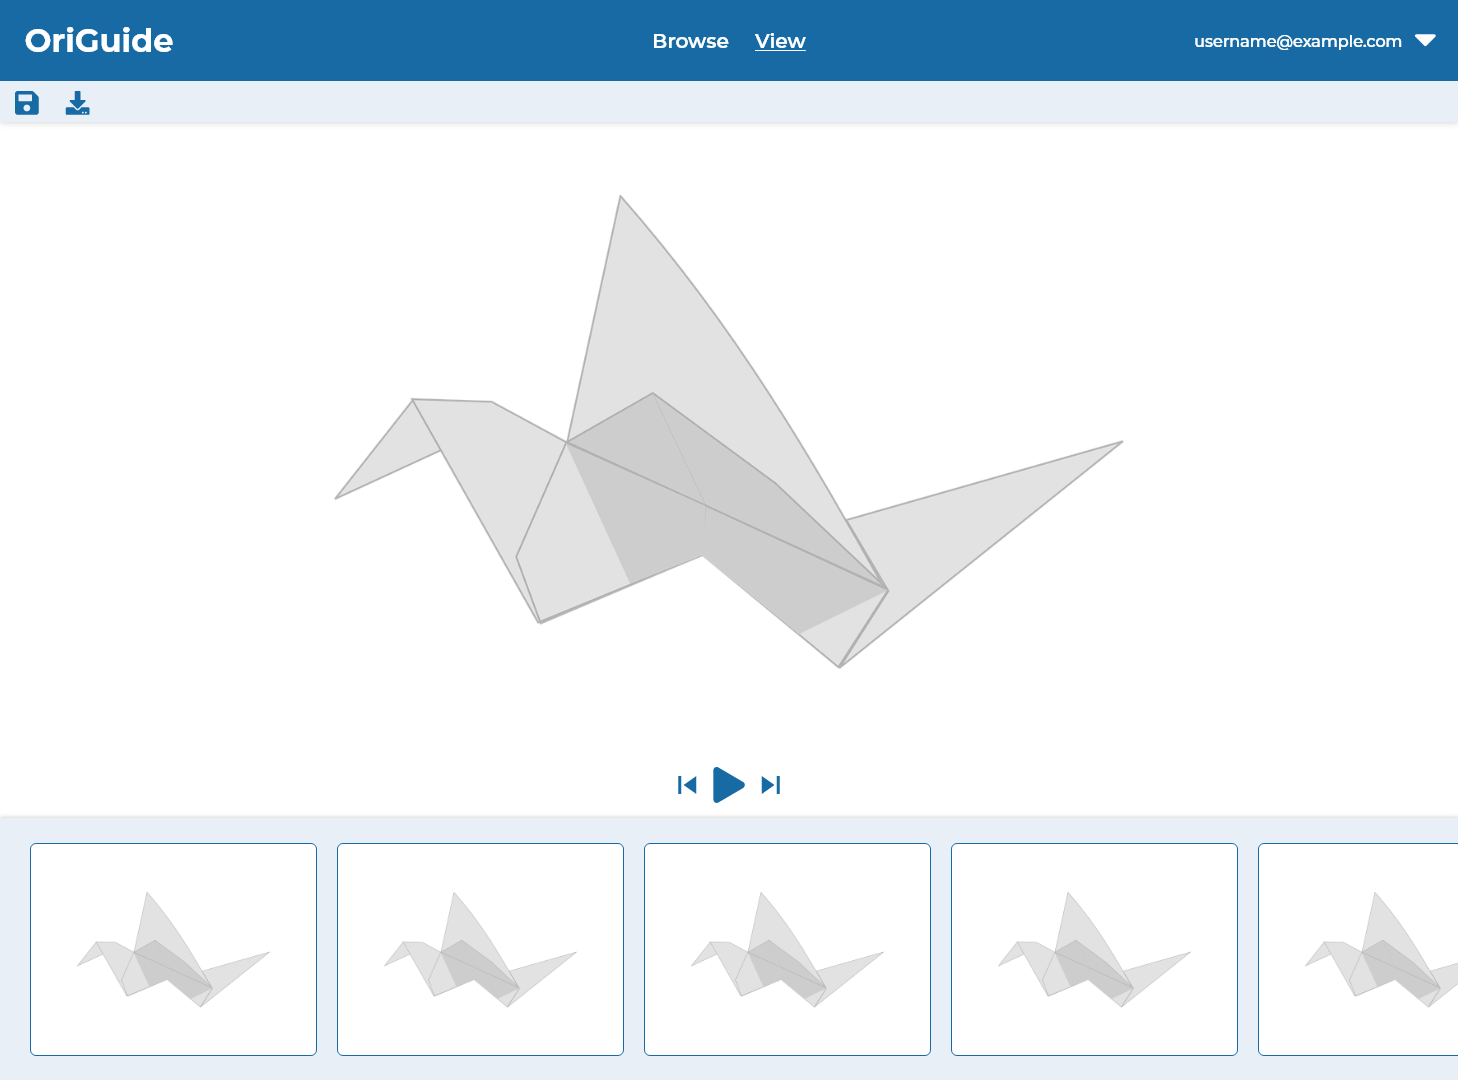
\includegraphics[width=0.8\textwidth]{assets/simulator-wireframe.png}
\end{figure}

\begin{figure}[H]
\caption{Community view}
  \centering
    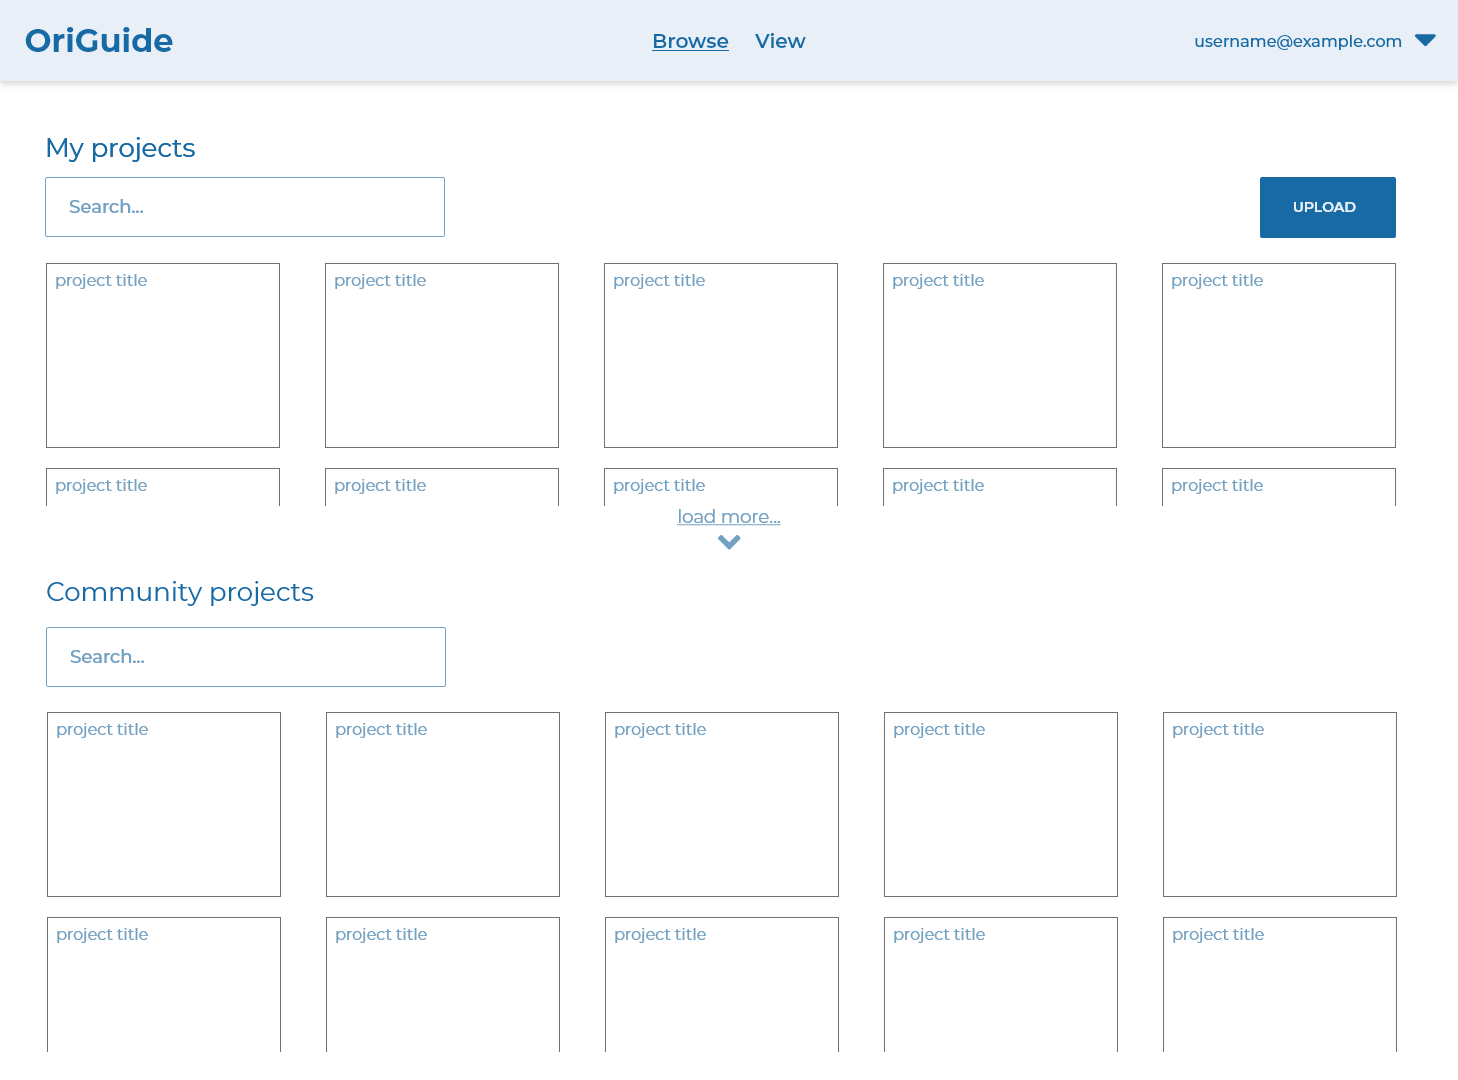
\includegraphics[width=0.8\textwidth]{assets/browser-wireframe.png}
\end{figure}


\section{\SectionTitleImplementationAspects}
\label{sec:implementation}
\subsection{Prototype}

From the list of features mentioned in the previous chapter we have selected the most important ones and created a prototype in a form of MVP (Minimum Viable Product). 

The selected features:

\begin{enumerate}
	\requirement{3}{load an Instruction}
	\requirement{3}{view the 3D representation of the Instruction step}
	\requirement{3}{switch to the next step in the Instruction}
	\requirement{3}{switch to the previous step in the Instruction}
	\requirement{3}{see the Transition between two Instruction steps}
	\requirement{2}{pause the Transition at any time}
	\requirement{2}{rewind the Transition}
	\requirement{2}{forward the Transition}
	\requirement{3}{rotate the Model in 3D space}
	\requirement{3}{zoom the Model in and out in 3D space}
	\requirement{1}{see creases of the Model} 
	\requirement{2}{distinguish paper's top and bottom sides} 
\end{enumerate}

Some of the listed functionalities require a numerical solver which is also included in the MVP.

Both Instructions and Transitions are represented using .fold files which we have extended with information required by the application.

\subsubsection{Frontend}

At first we had decided to use plain \tech{JavaScript} with the \tech{Rollup} bundler and \tech{Three.js} framework.
It quickly became apparent that the lack of state management will become problematic as the development progresses. Following that realization we have decided to incorporate a reactive framework - \tech{React} to aid the project with basic layout and aforementioned state manipulation. 
Due to minor interoperability issues the Rollup was also replaced with \tech{Webpack}.

The quality assurance is achieved through the use of:

\begin{description}
\item[Code linter] - EsLint
\item[Code prettiefier] - Prettier
\item[Test Runner] - Jest
\item[Continuous integration] - Github Actions
\end{description}

The implementation is continuously delivered to \tech{Netlify} via Github Actions.


\begin{figure}[H]
\caption{Origami simulation view}
  \centering
    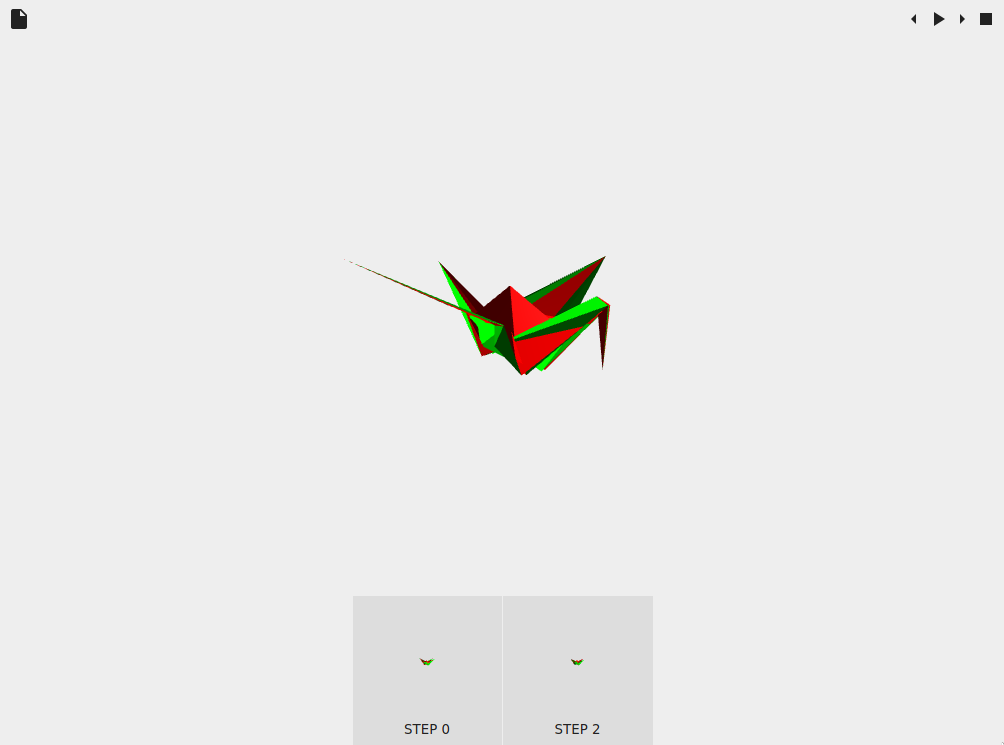
\includegraphics[width=0.8\textwidth]{assets/prototype-front.png}
\end{figure}

\subsubsection{Backend}

The current backend part is responsible for carrying out numerical computations.
It converts a provided Instruction into a set of coordinates representing
transitions between folding steps.\\

The solver is based on the techniques presented in the publication by A. Ghassaei.\cite{origami-simulator}.

The computational framework consists of the three most important forces,
that drive the folding process.

\begin{description}
	\item[Beam force] - responsible for preserving edge length
	\item[Face force] - responsible for preserving the original face shape
	\item[Crease force] - responsible for folding
\end{description}

Given the current vertices' positions, and the mountain-valley assignment,
the solver computes forces imposed on vertices, and calculates their next position
using the forward Euler integration.

An additional \textbf{damping force} is introduced to prevent solver from
high frequency oscilations, assuring numerical stability under most conditions.\\

The solver is implemented in \tech{python}, using \tech{numpy} and \tech{scipy} libraries. 


\begin{figure}[H]
	\caption{Visualization of vertices (dots), and forces applied to them (arrows)
	during folding of a rectangular sheet of paper in half, along the diagonal. }
  \centering
    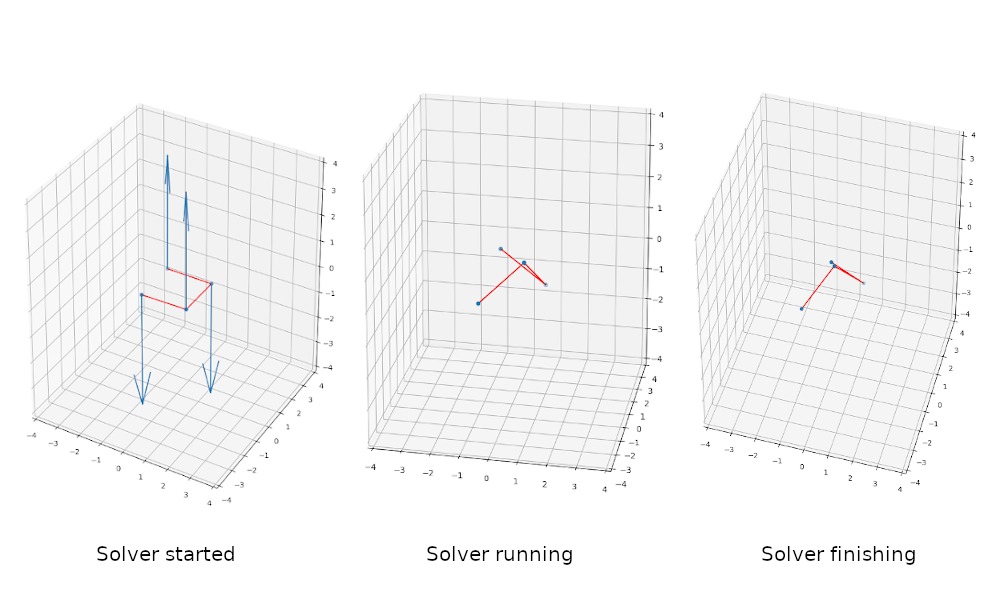
\includegraphics[width=0.8\textwidth]{assets/prototype-backend.png}
\end{figure}


\subsection{Project overview}

\begin{figure}[H]
	\caption{High level system overview}
  \centering
    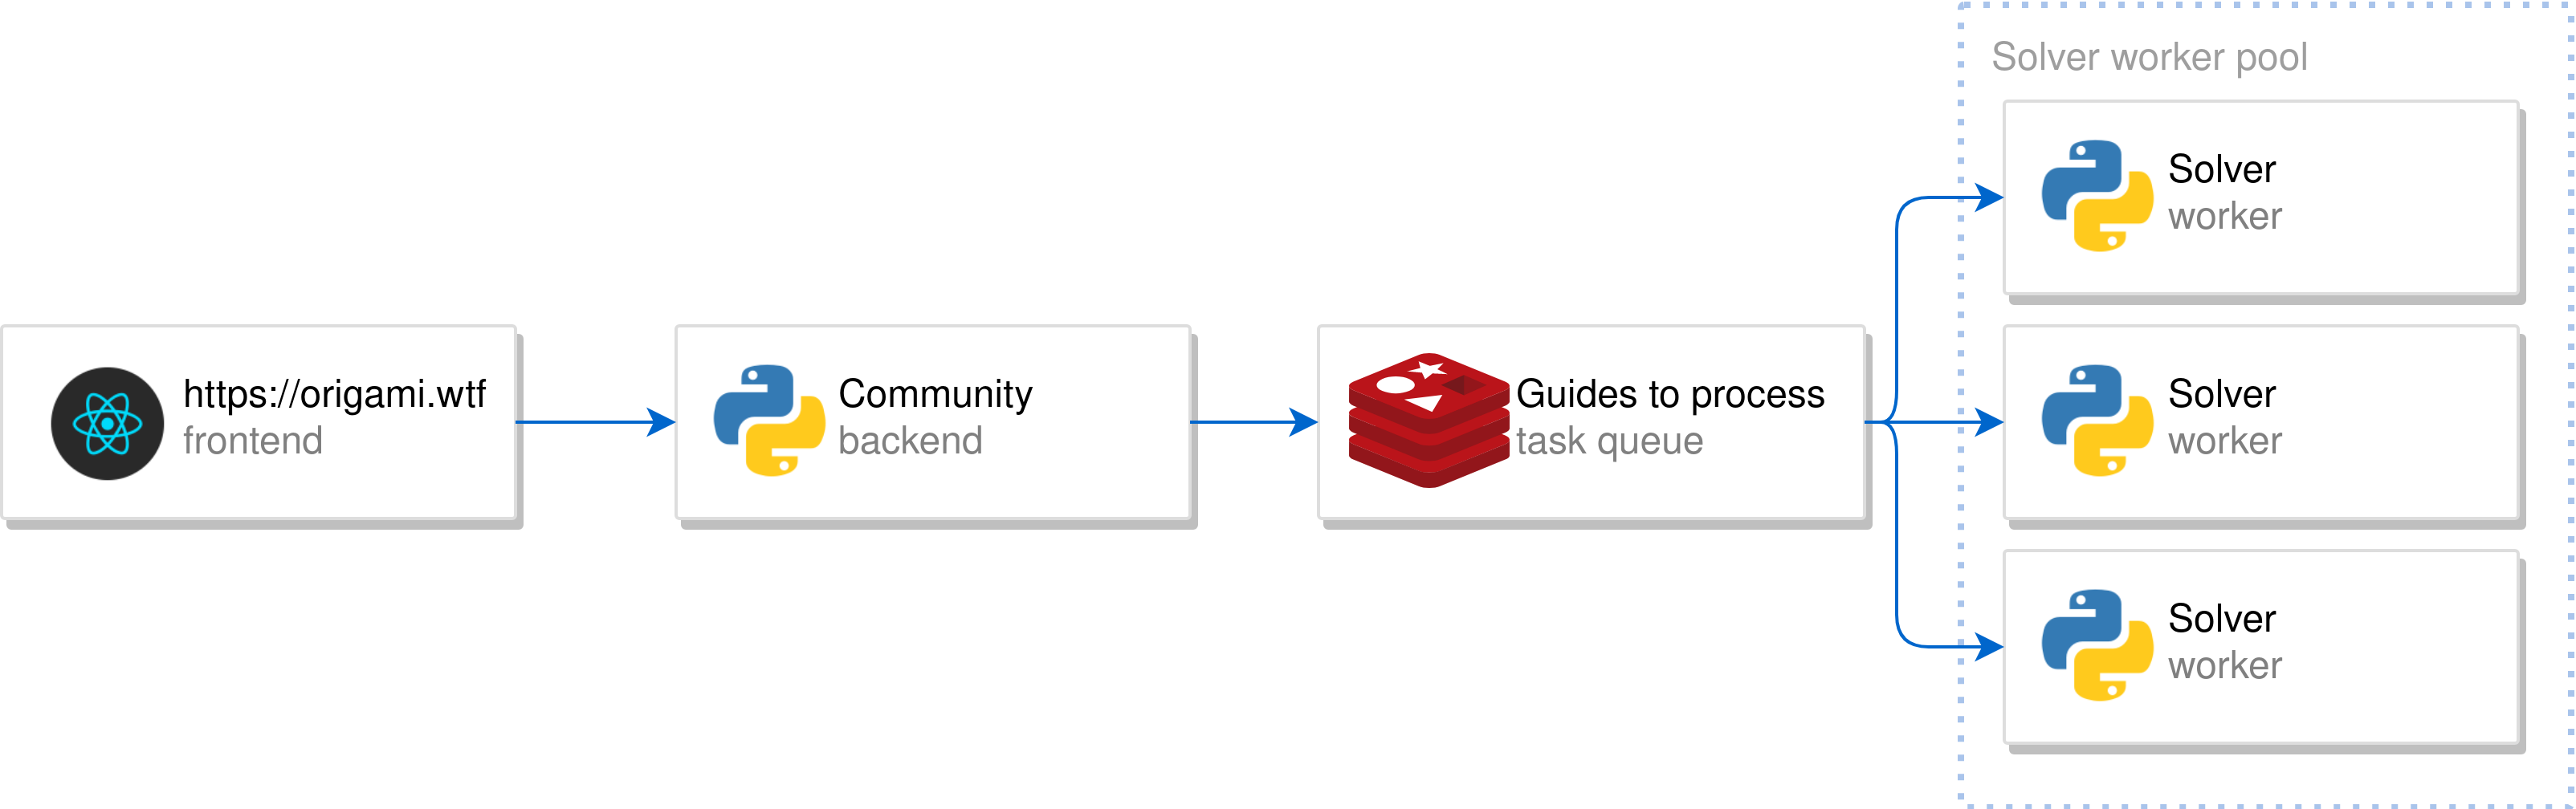
\includegraphics[width=\textwidth]{assets/architecture.png}
\end{figure}

Origuide consists of the following layers:
\begin{description}
	\item[Frontend] - a component that handles all user interactions with the system. 
	\item[Backend] - a component responsible for: \begin{itemize}
		\item processing all user requests initiated on the Frontend
		\item managing persistent data 
		\item authentication and authorization
		\item scheduling Guide processing
	\end{itemize}
	\item[Guides to process] - a task queue distributing guides to process among Solver workers
	\item[Solver worker] - a component responsible for converting Instructions to Guides.
\end{description}

As we previously distinguished two types of users in the system, there are two main success paths through the application.

\begin{figure}[H]
	\caption{Designer's success path}
  \centering
    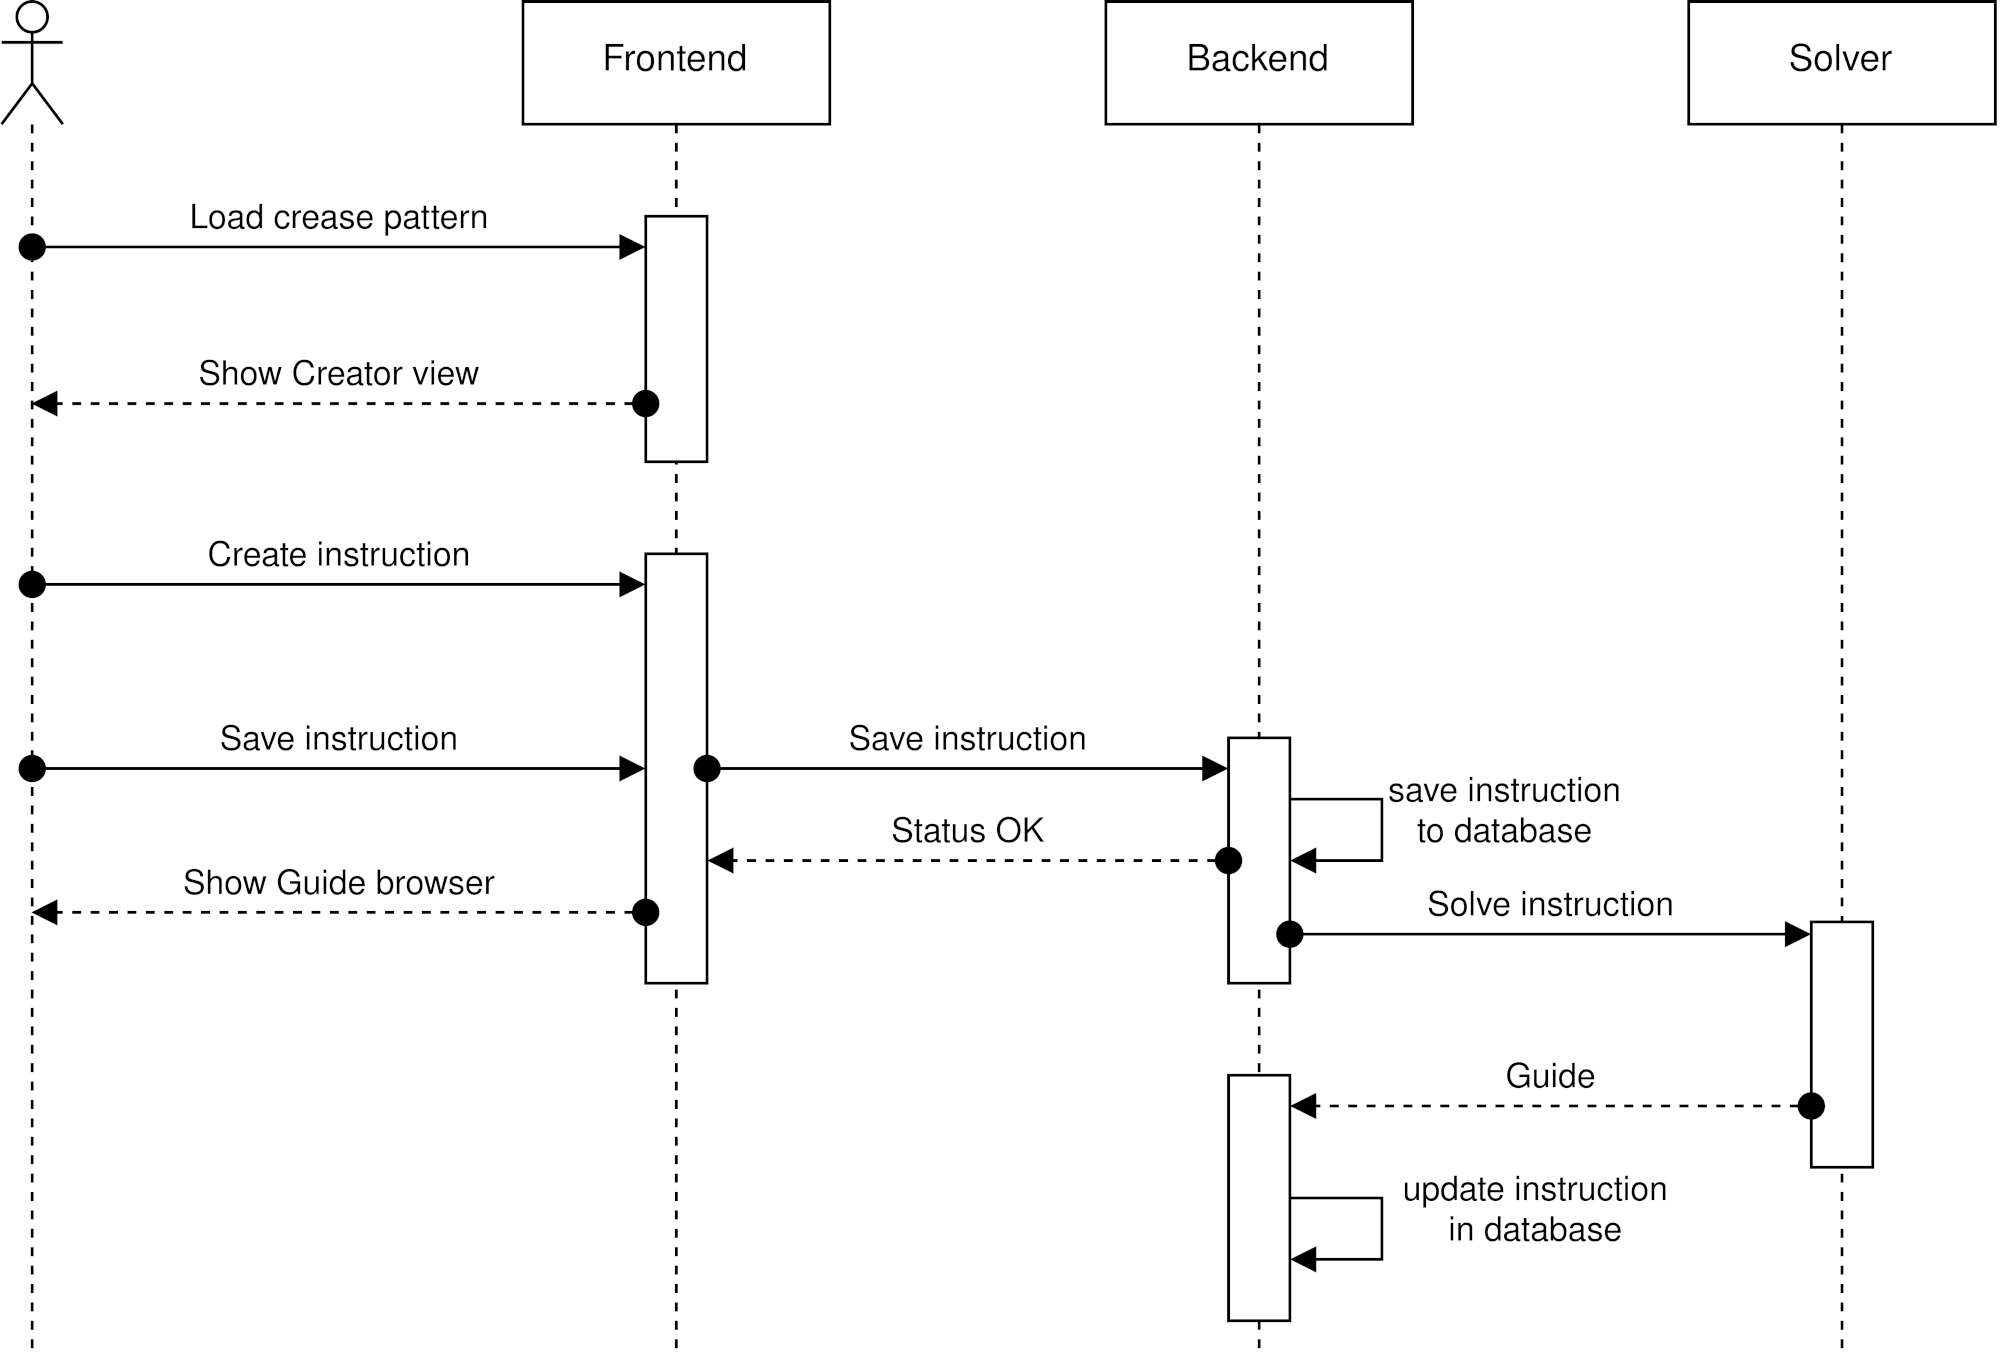
\includegraphics[width=\textwidth]{assets/3-designer-flow.png}
\end{figure}

Designer's main objective is to create Guides. After uploading a Crease Pattern, Designer is required to provide instruction steps. When an Instruction is saved it gets scheduled on a Task Queue and processed by a Solver worker. Once processing is finished the Instruction associatied with the Guide is marked as solved in the database.

\begin{figure}[H]
	\caption{Folder's success path}
  \centering
    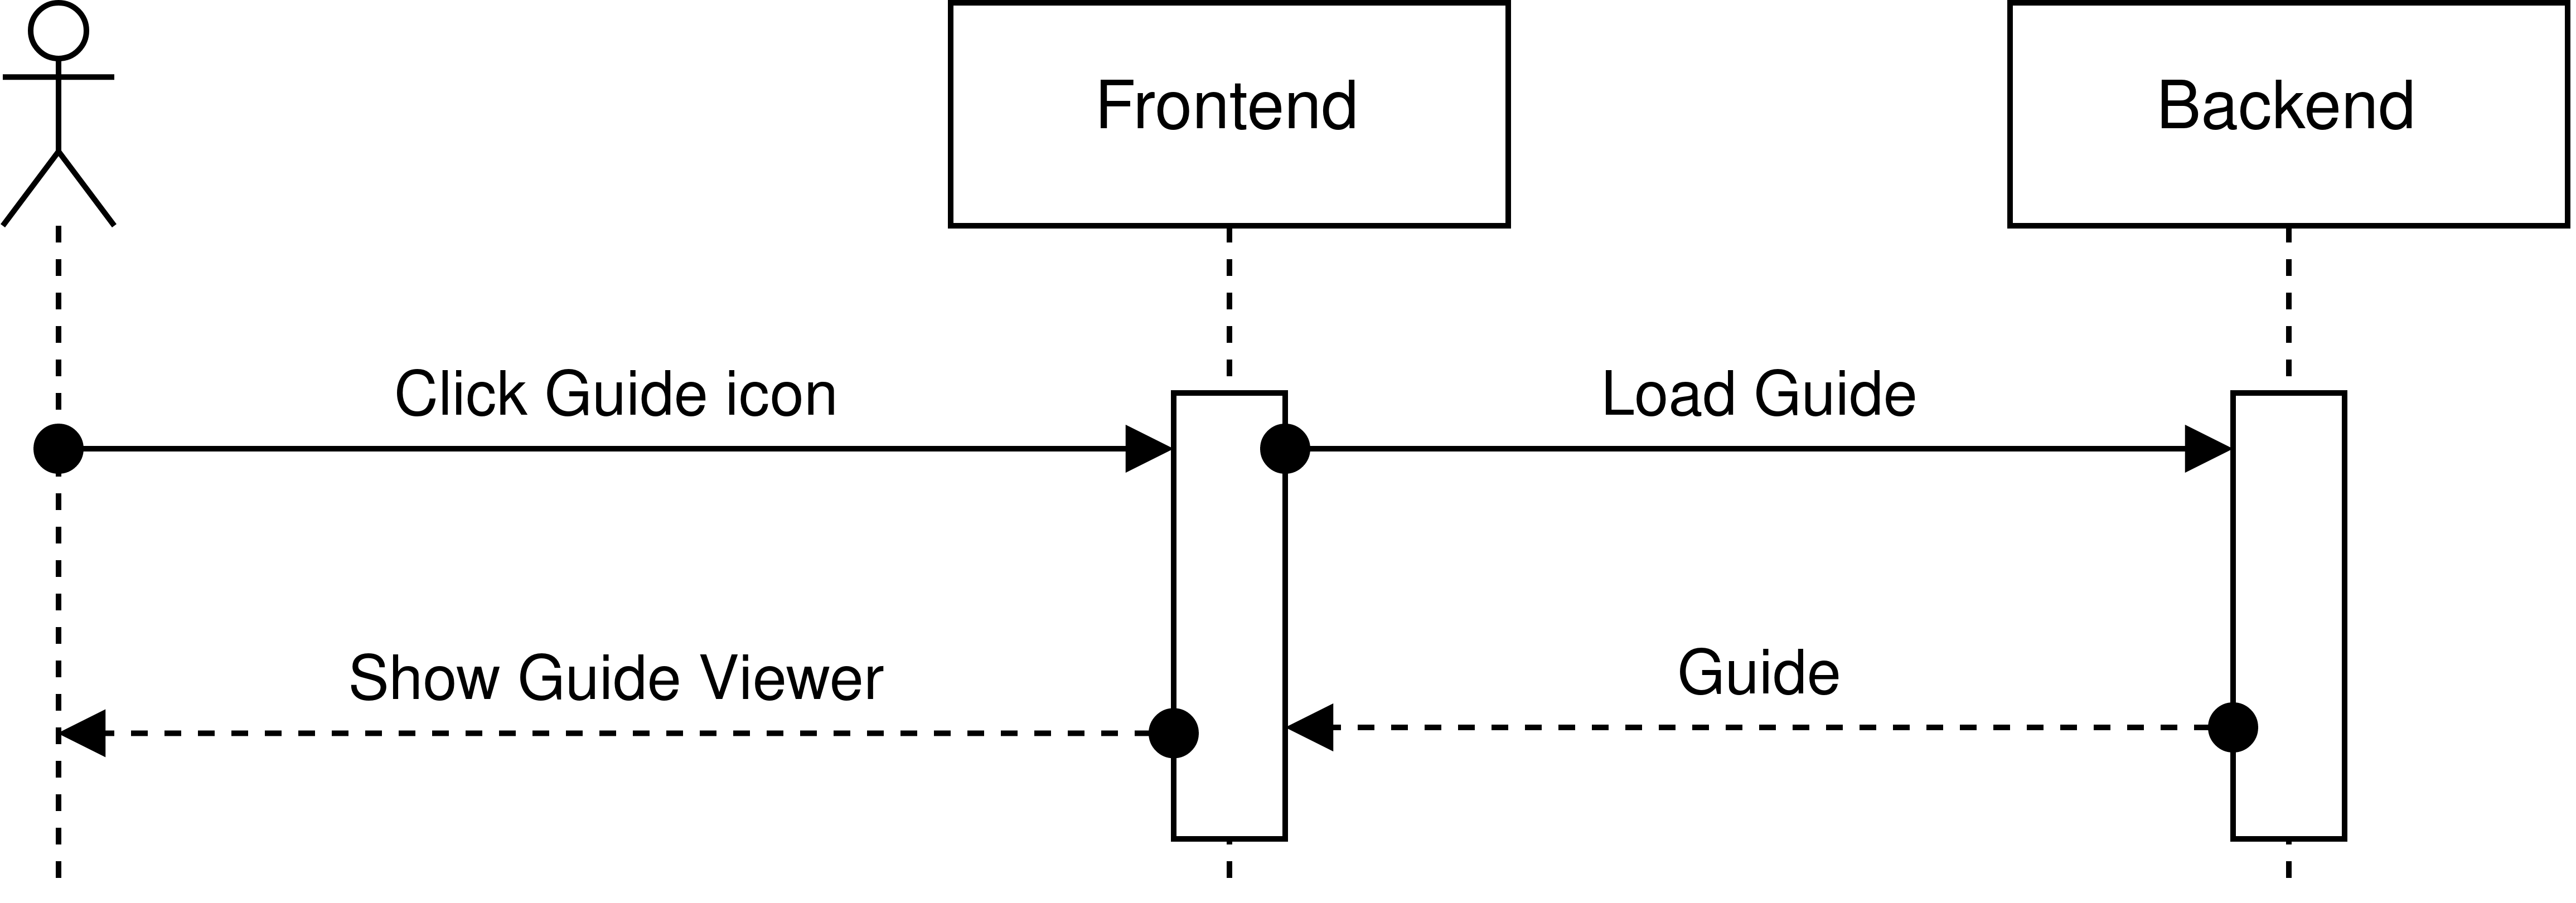
\includegraphics[width=\textwidth]{assets/3-folder-flow.png}
\end{figure}

Folder's main objective is to fold origami figures following steps presented by the Application. After successfully retrieving a guide from the Backend, he is presented with a Guide Viewer.

\subsection{Technology stack}

Source Code is version controlled using a hosted \tech{Git} solution - \tech{Github}.  

Continuous Integration and Continuous Deployment is provided by \tech{Github Actions}. 

\subsubsection{Frontend}

\begin{itemize}
	\item The Application is built in \tech{Javascript} using \tech{React} framework. 
	\item \tech{Three.JS} is used to display 3D models.
	\item Triangulation is done using \tech{earcut}. 
	\item Parsing folds is aided by \tech{fold}.
	\item User Interface components come mainly from \tech{material-ui}.
	\item \tech{Webpack} is responsible for bundling, minimizing and transpiling the source code.
	\item Code style is checked using \tech{Prettier} with \tech{eslint} and enforced on every commit using \tech{Husky}.
	\item \tech{Jest} has been incorporated as a test runner.
\end{itemize}

// TODO: comment

\subsubsection{Backend}

\begin{itemize}
	\item The Backend is built in \tech{Python} using \tech{Django} framework. 
	\item \tech{DjangoRestFramework} simplifies a REST server setup.
	\item \tech{drf-base64} helps with decoding of base64 encoded files.
	\item \tech{PyJWT} assists in auth process.
	\item \tech{factory-boy} is used to generate testing data.
	\item Data is stored in a \tech{PostgreSQL} database.
	\item \tech{Celery} was chosen for an asynchronous task processing.
	\item \tech{Redis} acts as a task queue for \tech{Celery}.
\end{itemize}


\subsubsection{Solver}

\begin{itemize}
	\item Solver runs under \tech{Python}'s alternative implementation - \tech{PyPy}.
	\item \tech{Shapely} is used for triangulation.
\end{itemize}



\subsection{Components overview}
% Przegląd poszczególnych komponentów a wiec np. baza danych, aplikacja typu klient, serwis RESTowy. Jeśli baza to ERD z opisem, jeśli aplikacja kliencka to jakie elementy, widoki, jak się łączy i kiedy. Jeśli prosta aplikacja WWW to można pokazać strukturę projektu. Jeśli serwis RESTowy to jego specyfikacja z przykładami. Protokół komunikacji to może być zupełnie osobny opis. %

\subsection{Algorithms}
% Ciekawsze algorytmy, aspekty, mechanizmy np. logowanie, indeksowane, cachowanie, synchronizacja, backup, jakieś procesy w tle, jakieś progress bary, jakieś analizy, generowanie warstw GISowych, lokalizacja etc. Jest tu często o czym pisać. %

\subsection{Development environment setup}
% Instrukcja postawienia środowiska deweloperskiego - jeśli potrzeba wypełniacza %

\subsection{Deployment}
% Instrukcja postawienia środowiska deweloperskiego - jeśli potrzeba wypełniacza %

\subsection{Quality assurance}
% Quality Assurance: czy mamy testy jednostkowe? Czy mamy inne testy automatyczne? Jakich bibliotek używacie? %
At every commit that is a part of the master branch or a Pull Request Unit Tests are run. \\

\subsection{Problems encountered}
% Z jakimi problemami technicznymi sie borykaliście? Jeśli nie opisaliście ich w dokumentacji procesowej. %


\clearpage

\section{\SectionTitleWorkOrganization}
\label{sec:organizacja-pracy}
\emph{} 
\clearpage

\section{\SectionTitleResults}
\label{sec:wyniki-projektu}
\emph{}  
\clearpage

\bibliography{bibliography}

\end{document}
